\documentclass[10pt,a4paper,parskip=half]{scrartcl}
\usepackage[utf8]{inputenc}
\usepackage[ngerman]{babel}
\usepackage[T1]{fontenc}
\usepackage{graphicx}
\usepackage{setspace}
\usepackage{enumitem}

\usepackage{geometry}
\geometry{a4paper,left=25mm,right=25mm,top=25mm,bottom=45mm}
\usepackage[
automark, % Kapitelangaben in Kopfzeile automatisch erstellen
headsepline, % Trennlinie unter Kopfzeile
ilines % Trennlinie linksbündig ausrichten
]{scrlayer-scrpage }

\useshorthands{+}
\defineshorthand{+S}{\Sentence\ignorespaces}
\defineshorthand{+.}{. \Sentence\ignorespaces}

\pagestyle{scrheadings}
\clearpairofpagestyles

% Kopfzeile
\renewcommand{\headfont}{\normalfont} % Schriftform der Kopfzeile
\ihead{Vereinsjugendordnung des Luftsportverein Degerfeld e.V.\\\textit{\headmark}}
\chead{\\[1ex]\scriptsize{25. Oktober 2023}}
\ohead{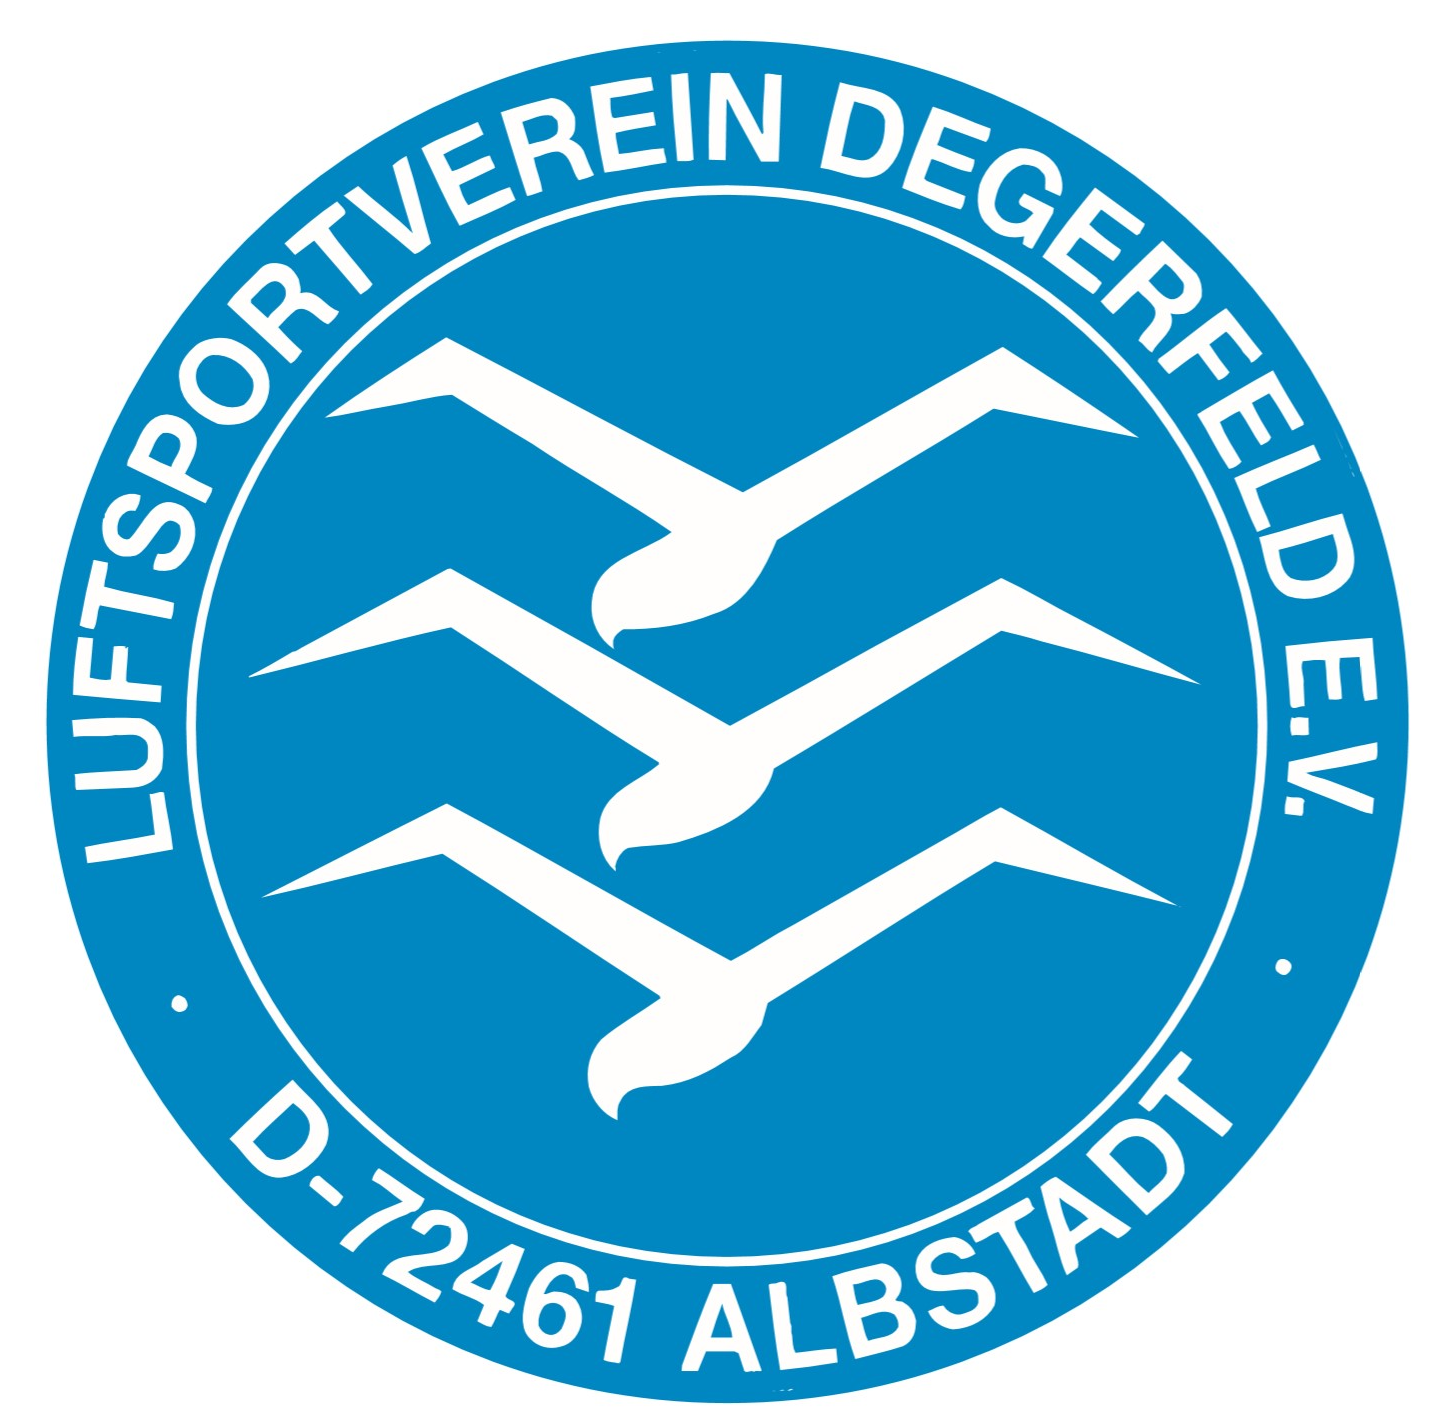
\includegraphics[scale=0.075]{../Logo.png}}
\setlength{\headheight}{20mm} % Höhe der Kopfzeile

% Fußzeile
\ifoot{\today}
\cfoot{}
\ofoot{\pagemark}
\setlength{\footskip}{20mm}

\frenchspacing % erzeugt ein wenig mehr Platz hinter einem Punkt
% Schusterjungen und Hurenkinder vermeiden
\clubpenalty = 10000
\widowpenalty = 10000
\displaywidowpenalty = 10000
\linespread{1.25} % Mehr Zeilenabstand

\usepackage{scrjura,multicol}
\setlength\columnsep{20pt} % Abstand zwischen den Spalten

\usepackage{helvet}
\addtokomafont{disposition}{\rmfamily} 
\addtokomafont{contract.Clause}{\rmfamily}
\renewcommand{\rmdefault}{phv}

\usepackage[hidelinks]{hyperref}

\title{Vereinsjugendordnung des Luftsportverein Degerfeld e.V.}
\subtitle{beschlossen am 25 März 2023}

\begin{document}

\thispagestyle{plain}
\begin{center}
  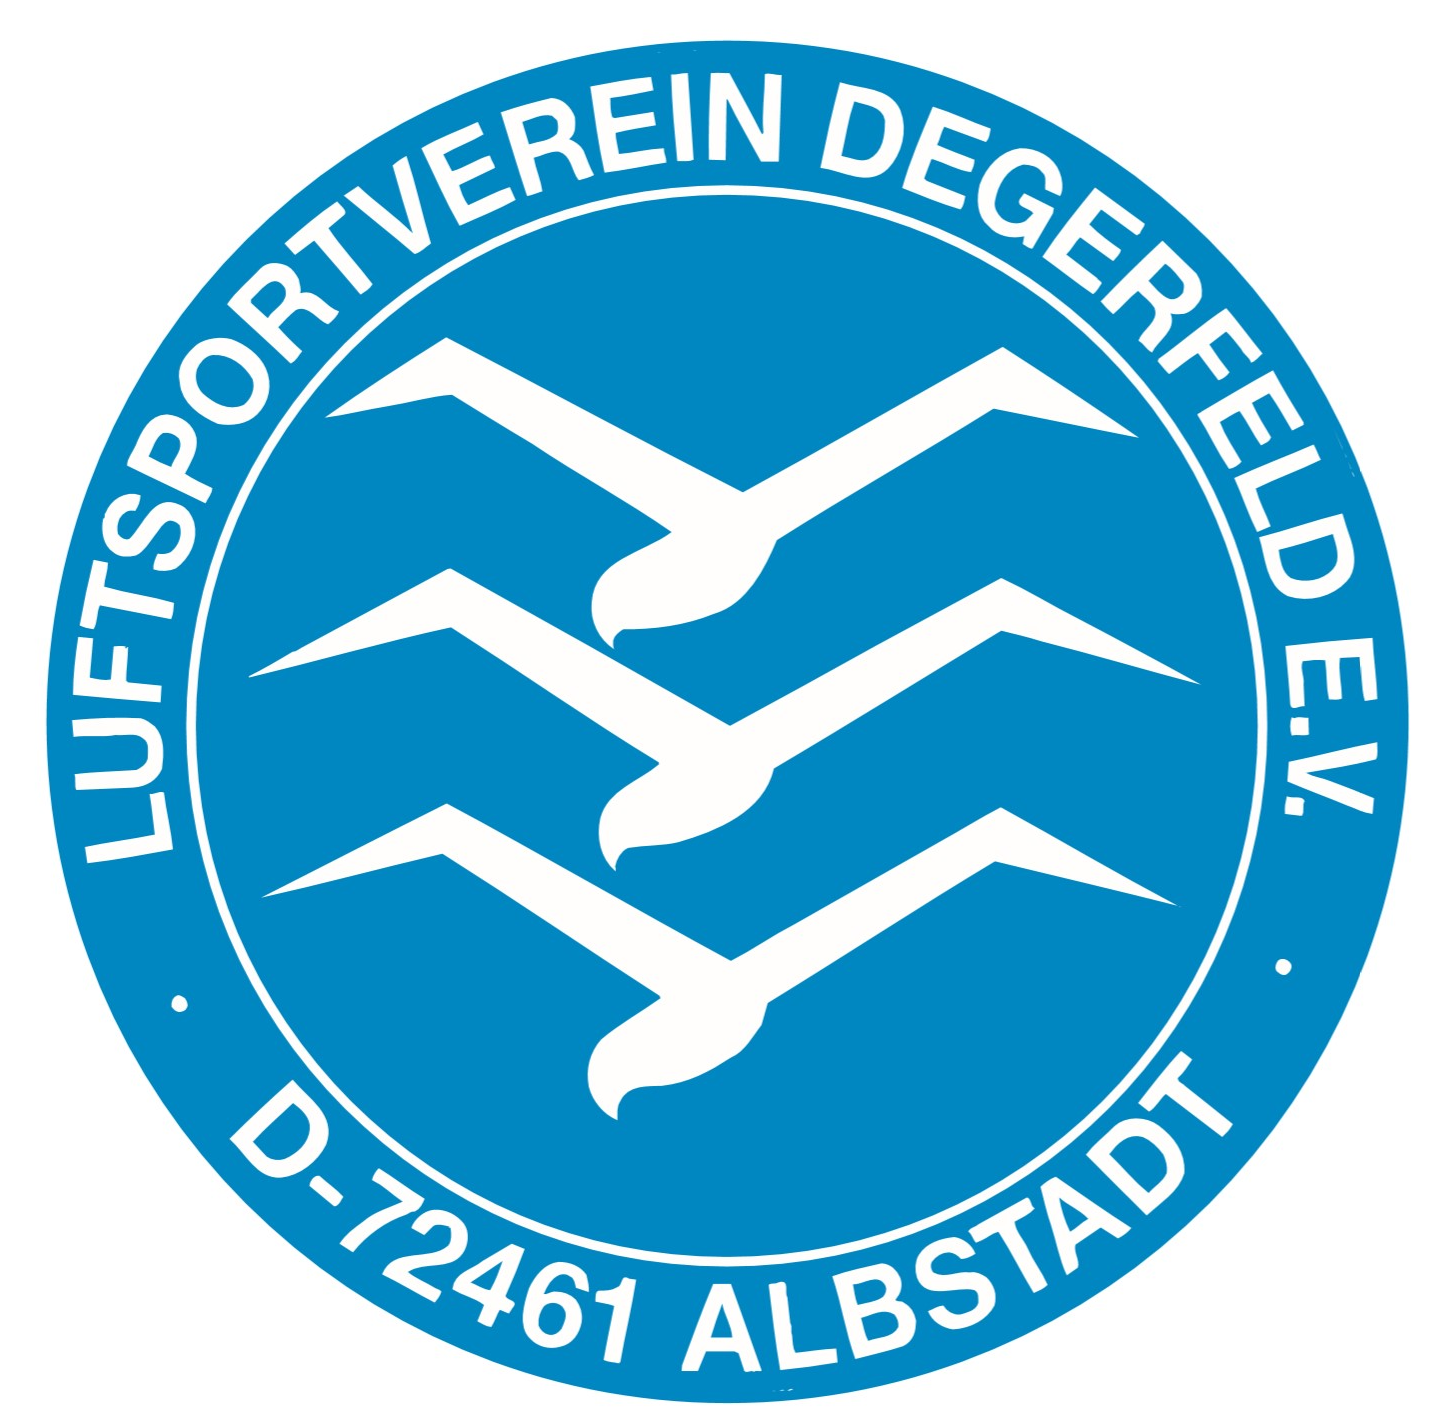
\includegraphics[scale=0.2]{../Logo.png}\\[5ex]
  
  \Huge{\textbf{Vereinsjugendordnung}}\\[1.5ex]
  \large{beschlossen am}\\[1.5ex]
  
  \normalsize
  
  \textbf{\Large{25 März 2023}}\\
  
\end{center}

\begin{contract}
  % \begin{multicols}{2}
    
    \Clause{title={Bezeichnung und Zugehörigkeit}}

    Der Luftsportverein Degerfeld unterhält in ihrem Rahmen eine Jugendgruppe unter dem Namen Luftsportjugend Degerfeld. Die Vereinsjugendgruppe ist dem Jugendverband des baden-württembergischen Luftfahrtverbandes (BWLV) angegliedert.
    
    Die Luftsportjugend wird freiwillig von allen Jugendlichen (Jugendliche Mitglieder sind Jugendliche im Sinne der Definition der Satzung des Vereins) gebildet, die Mitglied des Vereins und des BWLV sind.
    
    Die Vereinsjugendordnung ist eine Ergänzung zur Satzung des Luftsportverein Degerfeld. Die Bezirksjugendordnung und die Jugendordnung des BWLV bilden die Grundlage zur Vereinsjugendordnung.

    \Clause{title={Ziel und Aufgaben}}
    Ziel der Luftsportjugend ist es, neben der Pflege und Förderung des Luftsports, jugendfördernd und jugendpflegerisch zu wirken.

    \SubClause{title={Aufgaben}}

    Pflege und Förderung des Luftsports auf Vereinsebene durch Veranstaltung von Jugendwettbewerben und Jugendtreffen aller Luftsportarten des BWLV.

    Durchführung von Jugendfreizeiten, Seminaren und Lagern auf Vereinsebene.

    Förderung von Jugendbegegnungen auf nationaler und internationaler Ebene.

    Zusammenarbeit und Verhandlungsführung mit den zuständigen staatlichen und kommunalen Stellen, sowie mit allen in der Jugendarbeit stehenden Vereinen, Verbänden und Institutionen.
    
    Entwicklung von Initiativen für eine zeitgemäße und gesellschaftsbezogenen Jugendarbeit.

    Förderung und Durchführung geeigneter Maßnahmen zur Nachwuchsgewinnung

    \Clause{title={Organe}}

    Vereinsjugendversammlung

    Vereinsjugendleitung

    \Clause{title={Die Vereinsjugendversammlung}}

    Stimmberechtigt in der Vereinsjugendversammlung sind alle jugendlichen Mitglieder (Jugendliche im Sinne der Definition des Baden-Württembergischen Luftfahrtverbandes (BWLV), die dem BWLV gemeldet sind. Außerdem haben der Vereinsjugendleiter und sein Stellvertreter je eine Stimme.

    Die Vereinsjugendversammlung tritt jährlich mindestens einmal zusammen.

    Zur Vereinsjugendversammlung wird schriftlich 1 Monat vorher mit Tagesordnung vom Vereinsjugendleiter eingeladen.

    Anträge sind spätestens 1 Woche vor der Versammlung schriftlich an den Vereinsjugendleiter einzureichen.

    Über die Versammlung ist ein Protokoll zu führen. Zu Beginn der Versammlung ist ein Protokollführer zu bestimmen.

    \SubClause{title={Aufgaben}}
    
    Anregungen und Vorschläge zur Jugendarbeit im Verein.

    Beschlussfassung der Jugendordnung, Beschlussfassung über Änderungen der Jugendordnung und über die Anträge an die Versammlung.

    Wahl des Vereinsjugendleiters und seines Stellvertreters.

    \Clause{title={Die Vereinsjugendleitung}}

    Die Vereinsjugendleitung setzt sich zusammen aus dem Vereinsjugendleiter/-in und seinem Stellvertreter/-in.

    \SubClause{title={Aufgaben}}

    Geschäftsführung der Jugendgruppe im Verein.

    Vertretung der Vereinsjugend gegenüber dem Vereinsvorstand, Bezirksjugendleitung, Landesjugendleitung und Ämtern.

    Vertretung der Vereinsjugend in der Öffentlichkeit.

    Der Vereinsjugendleiter wird erforderlichenfalls durch seinem Stellvertreter vertreten.

    \Clause{title={Wahlverfahren}}

    Abstimmungen und Beschlüsse werden in einfacher Mehrheit der erschienenen Stimmberechtigten gefasst.

    Änderungen der Jugendordnung können nur mit 2/3-Mehrheit der erschienenen Stimmberechtigten vorgenommen werden. Auf die beabsichtigte Änderung ist in der Einladung hinzuweisen.

    Auf Antrag werden die Wahlen und Abstimmungen geheim durchgeführt.

    Die Wahl erfolgt auf zwei Jahre und sollte sich mit der Amtszeit des Vereinsvorstandes decken, Der Jugendleiter und sein Stellvertreter werden im jährlichen Wechsel gewählt.

    \Clause{title={Sportliche Betreuung}}

    Die flugsportliche und handwerkliche Betreuung der Jugendgruppe obliegt dem Ausbildungsleiter, den Fluglehrern und technischen Leitern des Flugsportvereins. Sie erfolgt nach den vom BWLV gegebenen Richtlinien für Flugbetrieb und Werkstattarbeit.

    \Clause{title={Beiträge, Kassen- und Rechnungswesen}}

    Die Beiträge der Jugendlichen beschränken sich auf den regulären Beitrag als ordentliche/ außerordentliche Mitglieder an den Flugsportverein. Darüber hinaus dürfen an die Jugendlichen keinerlei Beitragsforderungen gestellt werden.

    \SubClause{title={Jugendkasse}}

    Die Vereinsjugend wirtschaftet selbständig und eigenverantwortlich mit den ihr direkt zufließenden Jugendfördermitteln. Sie ist verantwortlicher Empfänger der Zuschüsse für jugendpflegerische Maßnahmen.

    Die Vereinsjugend ist für den Nachweis einer zweckentsprechenden und ordnungsgemäßen Verwendung der Jugendfördermittel verantwortlich.

    Die Führung der Kasse der Vereinsjugend obliegt der Vereinsjugendleitung. Die Jugendkasse ist jährlich mindestens einmal von den vom Verein gewählten Kassenprüfern zu prüfen.

    Die Jugendkasse ist Teil des Vereinsvermögens. Sie ist zum Jahresende mit der Kasse des Vereins abzustimmen.

    Die Vereinsjugendgruppe verpflichtet sich, den Behörden der Länder, des Regierungsbezirks, der Kreise und Gemeinden, die Mittel für die Jugendarbeit zur Verfügung stellen, alle Nachweise zu geben, aus denen die ordnungsgemäße Verwendung zu ersehen ist.\\[10ex]

% \end{multicols}
\end{contract}
Jugendordnung beschlossen am 25.03.2023 durch den Ausschuss am xx.04.2023 verabschiedet.

\end{document}